\documentclass{article}

\usepackage{tikz}
\usepackage{svg}
\usetikzlibrary{shapes.geometric, arrows}

\tikzstyle{startstop} = [rectangle, rounded corners, minimum width=2cm, minimum height=1cm,text centered, draw=black, fill=red!30]
\tikzstyle{process} = [rectangle, minimum width=2cm, minimum height=1cm, text centered, draw=black, fill=blue!20]
\tikzstyle{arrow} = [thick,->,>=stealth]
\tikzstyle{sum} = [circle, minimum size=1cm, text centered, draw=black, node contents={\textbf{+}}]

%\usepackage[margin=1in]{geometry}
\usepackage{graphicx} % Required for inserting images
\usepackage{hyperref}
\usepackage{amsmath}
\usepackage{titling}
\usepackage{enumitem}
\usepackage{makecell}
\usepackage{minted}
\usepackage{url}
\usepackage{tabularx}
\usepackage{graphicx}
\renewcommand\maketitlehooka{\null\mbox{}\vfill}
\renewcommand\maketitlehookd{\vfill\null}

\begin{document}
\centering

\title{\Huge Intro IoT Machine Learning Project 1}

\author{ \huge
Jaskin Kabir \\
\Large Student Id: 801186717 \\
\Large \href{https://github.com/holleman-courses/proj1-awesome_team/}{GitHub:}\\\url{https://github.com/holleman-courses/proj1-awesome_team/}
}

\date{March 2025}

\begin{titlingpage}
\maketitle
\end{titlingpage}
\raggedright

\section{Introduction}
% Describe the purpose of the project, what you
%intended to accomplish, and inform the reader about the upcoming
%sections.  Two to three paragraphs should be sufficient.

The purpose of this project was to develop a machine
learning model capable of recognizing pencils and deploy
this model to the Arduino Nano 33 BLE Sense. This project
aims to demonstrate the feasibility of deploying a machine
learning model on embedded hardware with limited
computational resources. By focusing on a simple object like
a pencil, the project provides a manageable starting point
for exploring the challenges of embedded machine learning,
such as memory constraints, inference speed, and accuracy.

The intention is to produce a system that is not only
sufficiently accurate but also fast enough to be used in
real-time applications. The project involves designing a
neural network architecture that balances performance and
resource efficiency, constructing a dataset tailored to the
target object, and training the model to achieve optimal
accuracy. The upcoming sections will delve into the details
of the model architecture, the dataset preparation process,
the training methodology, and the results obtained. These
sections will also discuss the challenges encountered, and
the lessons learned during the development and deployment of
the system.

\section{Model Architecture}
For image classification on embedded hardware, the most
widely used paradigm is the convolutional neural network,
which was used in this project. As for the structure of the
network itself, a choice was made between a wide and short
network or a narrow and deep network. A wide and short
network would have few convolutional layers with each layer
consisting of many convolutional filters, whereas the deep
and narrow network would have many layers with fewer filters
in each layer. To allow for the greatest abstraction from
the input images, the narrow and deep network was chosen. To
resolve the issue of vanishing gradients, skip connections
were added between every two convolutional layers after the
initial layer. 

Each residual block consists of two convolutional layers
with batch normalization and relu activation functions
between them. The structure of the resblock can be seen in
Figure \ref{fig:resblock}. The overall network
topology is shown in Figure \ref{fig:network}. The initial
convolution uses a stride of 4 to reduce the size of the
input image so the microprocessor could process it. After
the initial convolution, the stride is set to 1 for the rest
of the network. The size of the network was mainly
constrained by the runtime, as the required tensor arena
size had to fit within the small RAM of the Arduino. The
parameter count was kept low enough to allow for faster
training and inference times, but large enough to accurately
classify images. To keep the required arena size low, the
maximum number of filters in each layer was kept at 128, and
on either side of the 128 filter layers is a 64 filter
layer.


\begin{figure}[ht]
\begin{center}
    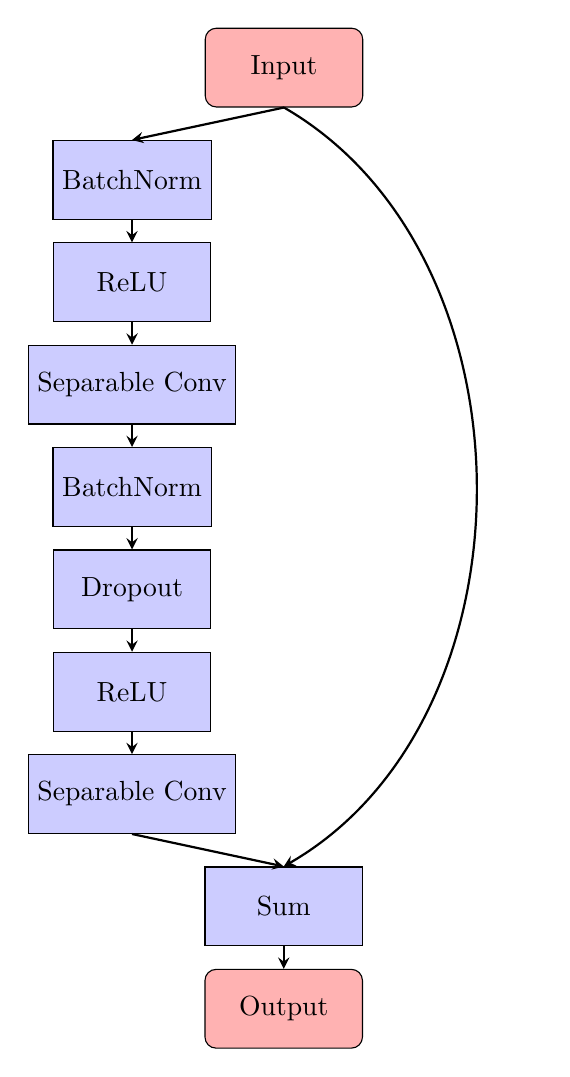
\begin{tikzpicture}[node distance=1.3cm]
        \node (input) [startstop] {Input};
        \node (bn1) [process, below left of=input, anchor = north east] {BatchNorm};
        \node (relu1) [process, below of=bn1] {ReLU};
        \node (sepconv) [process, below of=relu1] {Separable Conv};
        \node (bn2) [process, below of=sepconv] {BatchNorm};
        \node (dropout) [process, below of=bn2] {Dropout};
        \node (relu2) [process, below of=dropout] {ReLU};
        \node (conv2) [process, below of=relu2] {Separable Conv};
        \node (sum) [process, below right of=conv2, anchor = north west] {Sum};
        \node (output) [startstop, below of=sum] {Output};
        
        % Arrows for forward path
        \draw [arrow] (input.south) -- (bn1.north);
        \draw [arrow] (bn1.south) -- (relu1.north);
        \draw [arrow] (relu1.south) -- (sepconv.north);
        \draw [arrow] (sepconv.south) -- (bn2.north);
        \draw [arrow] (bn2.south) -- (dropout.north);
        \draw [arrow] (dropout.south) -- (relu2.north);
        \draw [arrow] (relu2.south) -- (conv2.north);
        % Residual connection
        %\draw [arrow] (input.east) -- ++(2cm,0) -- ++(0,-5.5cm) -- (conv2.east);
        \draw [arrow] (input.south) to [out=-30,in=30] (sum.north);
        
        % sum arrow
        \draw [arrow] (conv2.south) -- (sum.north);
        \draw [arrow] (sum.south) -- (output.north);
    \end{tikzpicture}
    \caption{Residual block}
    \label{fig:resblock}
\end{center}
\end{figure}

\begin{figure}[ht]
    \begin{center}
    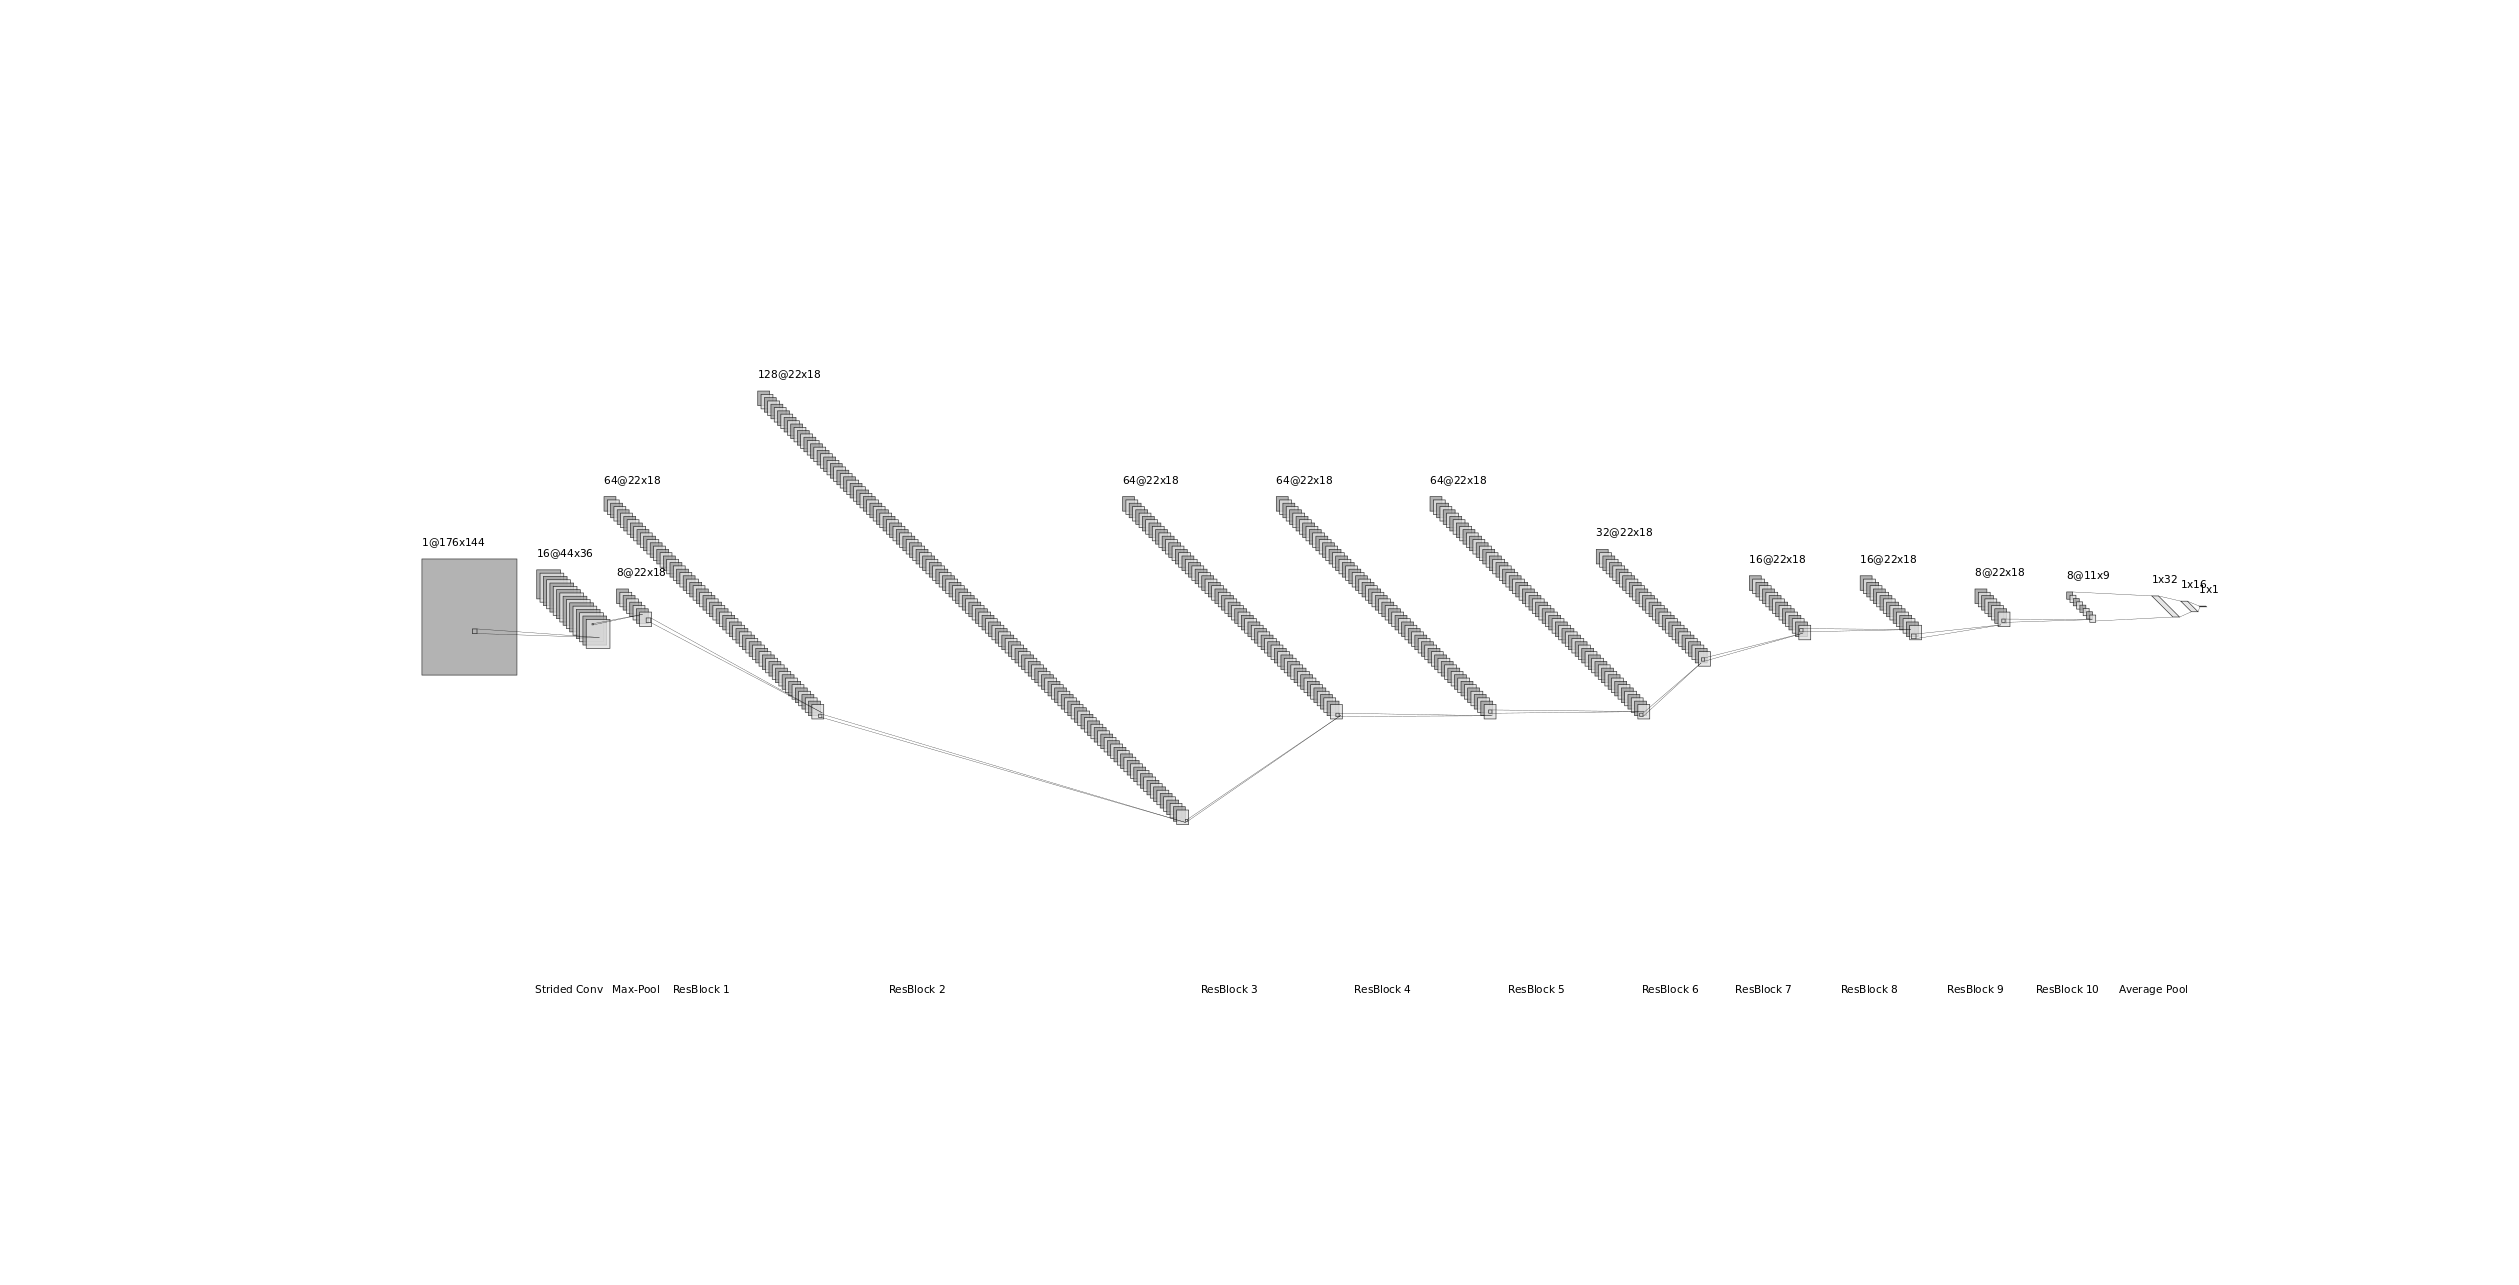
\includegraphics[width=350pt,height=175pt]{images/nn.png}
    \caption{Network topology}
    \label{fig:network}
    \end{center}
\end{figure}

\section{Data and Training}
The dataset used to train and evaluate the model was a set
of 896 grayscale images taken using the Arduino Nano and the
OV767X camera included in the kit. The images were taken at
a 176x144 resolution and manually labeled. The images
include pictures on various surfaces like chairs, jackets,
bedsheets and tables. 459 images contained a pencil and 437
did not. Of these negative images, some contained pictures
of screwdrivers or wrenches so that the model would not
learn to classify straight objects as pencils.

The images weren't resized or preprocessed in any way, other
than random rotation and flipping for data augmentation. The
images were not resized before training so that rescaling
logic wouldn't need to be implemented on the Arduino. The
dataset was split into a training set of 70\% and a
validation set of 30\%. The model was trained for 100
epochs, with a batch size of 32. The model was trained using
the Adam optimizer with a learning rate of 0.005. As seen in
Figure \ref{fig:loss}, the model suffered from significant
overfitting. Additionally, the validation curves are very
unstable. This is likely due to the small validation
dataset.

\begin{figure}[h]
    \begin{center}
    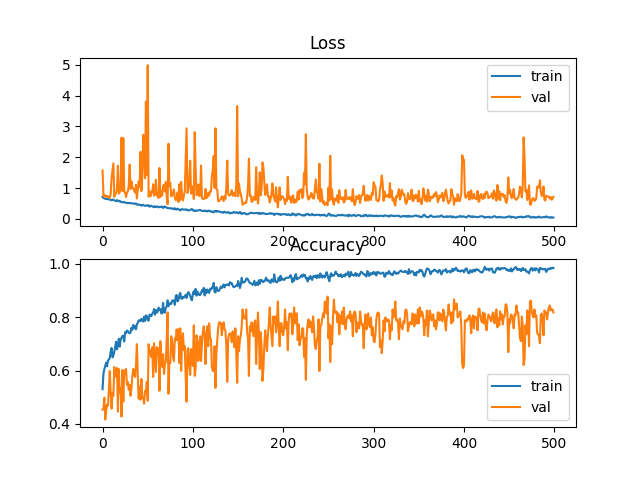
\includegraphics[width=320pt,height=240pt]{images/training.png}
    \caption{Loss and accuracy curves}
    \label{fig:loss}
    \end{center}
\end{figure}

\section{Results}
In software, the validation accuracy was 88\%. When deployed
to the Arduino, the system did respond to the target object,
but false positives were easy to induce. When pointed at a
granite countertop with a striped pattern, the stripes were
likely mistaken for pencils. Additionally, the model tends
to classify wires as pencils as well. This may have been
alleviated if more pencil-like objects were included in the
negative dataset.

Inference takes 4.883 seconds per image. The frame rate of
the camera was set to 5fps, as the dataset images were
captured at that frame rate to reduce blurriness. 
\newpage
\section{Summary Table}

\begin{table}[h]
    \begin{center}
    \begin{tabular}{|c|c|}
    \hline
    \textbf{Metric} & \textbf{Value} \\
    \hline
    Validation Accuracy & 87.73\% \\
    \hline
    Training Accuracy & 95.07\% \\
    \hline
    Inference Time & 4.883s \\
    \hline
    False Rejection Rate & 16.33\% \\
    \hline
    False Positive Rate & 7.38\% \\
    \hline
    Parameter Count & 112634 \\
    \hline
    Input Shape & 176x144x1 \\
    \hline
    MACs & 40,278,240 \\
    \hline
    Frame Rate & 5fps \\
    \hline
    \end{tabular}
    \caption{Summary of results}
    \label{tab:summary}
    \end{center}
\end{table}

\section{Discussion}
Overall, the system developed is a good proof of concept. It
successfully deploys a resnet based object detection model
that does respond to the target class. However, the
inference time is very slow, and the accuracy leaves much to
be desired. As the system takes almost 5 seconds to process
images, it would not be useful in real-time applications.
The biggest challenge was handling the small dataset.
Augmentation can only go so far, and the lack of validation
or test data led to unstable results. Thus, the first step
that should be taken to improve the system would to
collecting more data. To improve inference time, a much
shallower model should be used with fewer parameters.
\section{Conclusion}
Through this project, I learned how to deploy an object
detection model on an embedded system. I learned how to
construct a dataset and label it. I also learned how to
design a model's architecture to fit within the constraints
of the hardware. I learned how to train a model and evaluate
its performance. I also learned how to deploy a model to an
embedded system and measure its performance. This was the
biggest challenge, as many times I would build a model, but
it would fail upon deployment due to memory constraints.

\end{document}